\documentclass{llncs}
\usepackage[utf8]{inputenc}
\usepackage{tikz}
\usepackage[simplified]{pgf-umlcd}
\usepackage{cite}
\usepackage{listings}
%
\begin{document}

\title{LongXact: Making Long-Lived Transactions Easier to Develop}

%% Title
\author{João Pedro Carvalho}
\institute{Técnico de Lisboa/Universidade Técnica de Lisboa
\email{joao.pedro.carvalho@ist.utl.pt}}
\maketitle

%% Abstract

\begin{abstract}
Over the past years, Software Transactional Memories have become more
and more popular, growing to be something more than simply a research topic. On top of
that, the concept has been extended to encompass persistence, so
the concept of Persistent Software Transactional Memories was born. In
this thesis, I propose an extension to PSTM's in order to support the
concept of Long-Lived Transactions. Some research on the topic has
been conducted in the field of Database Transactions and Workflow
systems. My thesis is that supporting Long-Lived Transactions should
be done at the infrastructural level on Persistent STM's, so this
paper will describe how those systems can be extended to support
Long-Lived Transactions.
\end{abstract}

%% Intro

\section{Introduction}

For many years, enterprise applications were developed using
two-tiered architectures. In such architectures, there was typically a
mainframe with great computational power.

Long-Lived Transactions were first described in
1981 as ``[..] transactions with lifetimes of a few days or
weeks''\cite{gray1981transaction}. At the time, the author said that the
solution for this 

In this project, I aim at adding support for Long-Lived Transactions
in applications with Rich Domain Models.
Rich Domain Models are ``An object model of the domain that
incorporates both behavior and data.``, as described by \cite{fowler2003patterns}.

\section{Long-Lived Transactions}

\subsection{What are Long-Lived Transactions?}
\label{sec:what}

As previously described, Long-Lived Transactions are transactions with
a lifetime larger than a typical database transaction. In order to
better understand this concept, consider the following example, found
in the applications of many education institutions.

\begin{figure}
\centering
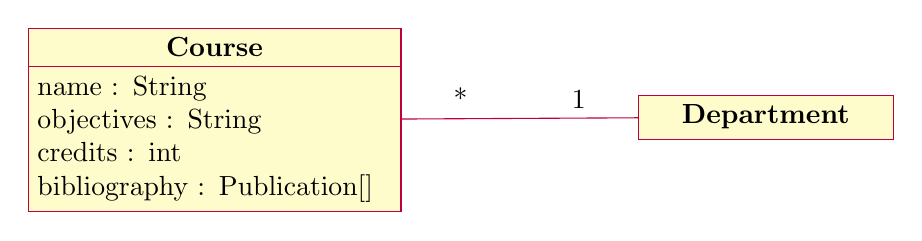
\begin{tikzpicture}

\begin{class}[text width=4.5cm]{Course}{0.5,0}
\attribute{name : String}
\attribute{objectives : String}
\attribute{credits : int}
\attribute{bibliography : Publication[]}
\end{class}

\begin{class}[text width=3cm]{Department}{7.5,-0.85}
\end{class}

\association{Department}{}{1}{Course}{}{*}

\end{tikzpicture}

\caption{Sample Domain Model in UML} 
\label{fig:courseDomain}

\end{figure}

In the domain model presented in Figure~\ref{fig:courseDomain}, we
present a simplification of the Course's attributes. A course belongs
to a department, has a name, its objectives, the credits granted upon
completion, and the recommended bibliography. The domain is deemed to
be consistent only if all attributes of Course have a defined value,
and each course must have a department. Each department is responsible
for managing its courses, meaning that it is up to someone who belongs
to the department to start the process of creating new courses.

Note that the creation of a new course should be executed
transactionally, since it is not desired that other users of the
system are able to see a course in an inconsistent state (either not
connected to any departement and/or without all attributes properly defined).

The pseudo-code in Listing~\ref{fig:courseCreation} implements the
business operation of creating a new course. Assume that {\bf
  department} is inferred from the user performing the operation. 

\lstset{language=Java,
basicstyle=\ttfamily,
stepnumber=2,
numbersep=9pt,
tabsize=4,
frame=single,
caption={Pseudo-Code for the
    creation of a new course. A new Course is created, associated with
  its department, and its attributes are filled.},
label={fig:courseCreation},
captionpos=b}
\begin{lstlisting}
Course course = new Course();
department.addCourse(course);
course.setName(name);
course.setObjectives(objectives);
course.setCredits(credits);
course.setBibliography(bibliography);
\end{lstlisting}

There are several ways to implement this operation. I will now
describe two common scenarios for said implementation.

\subsubsection{Business Transaction in a single interaction}

A possible implementation (most likely, the simplest) of the course
creation operation in a web application is to have a single page in
which the user provides all the required information. Once the
information is submitted, a new Course is created, associated with the
department of the person performing the operation, and all its
attributes are filled according to the information submitted by the
user. The new object is then stored in the database, making it
persistent and available for other users to view.

In this scenario, in which all the information can be provided in a
single user interaction, the transactional guarantees of the operation are
assured by the underlying database (which is assumed to provide the
classic transactional semantics \cite{gray1981transaction}), since the
whole operation can be performed within the scope of a single database
transaction.

An important consequence of implementing the operation in a single
database transaction is that the programmer can manipulate all the domain
objects involved directly. The order in which the modifications to
said objects are performed is irrelevant, as long as the domain is
consistent when the transactions is committed. This is the semantics
typically expected by a programmer of such applications: there may be
instants in which some domain objects are in an inconsistent state
(e.g. before defining the course's bibliography), however this
inconsistent state will never be seen by the other users of the
application. Those users will only see the fully created object once
the operation is committed.

\subsubsection{Business Transaction across multiple interactions}

The model described in the previous scenario, while simple and easy to
implement, may not be suited for every situation. Imagine that instead
of four attributes, Course had 50 attributes. It would then be
unfeasible to ask the user to fill everything out in a single web
page, so the logical solution would be to split the various attributes
in multiple pages, accounting for multiple interactions.

Let us now assume that the creation of a course is made throughout
three interactions. In the first interaction, the user selects the
course's name, in the second interaction, the user introduces the
objectives and credits, and in the final interaction, the user selects
the bibliography, thus creating the course.

At first glance, it would seem quite easy for a programmer to change
the logic programmed in the first scenario, in order to meet the new
requirements: the programmer would simply have to split the code
performed in a single request into three smaller parts, one to be
executed in each request.

However, having three separate requests implies three different
database transactions, breaking the atomicity and isolation of the
operation. After handling the first request, the persisted domain
would be in an inconsistent state (a course with no attributes but its
name).

The implementation of the business logic must then take this issue
into account, since the programmer cannot write the updates directly
on the domain, requiring manual handling.

This scenario represents what was defined as a Long-Lived Transaction,
in which the Business Operation had a larger lifetime that a single
database transaction (in this particular case, three database transactions).

\subsection{Why are they difficult to implement?}

Web frameworks provide a wide range of features to the
programmer. 

Transactional support, however, is still somewhat raw in most
Frameworks. Typically, transactions are handled by some database
beneath them, so the framework is just a thin layer, delegating all
the work.

Revisiting the example presented in \ref{sec:what}, there are several
ways to implement the second case (in which user interaction is made
in several steps).

\begin{enumerate}
\item Keeping a database transaction open during all the steps of the
  operation

\item Create a parallel representation of the objects that are being
  manipulated, store them outside the domain, and applying the changes
  only in the last interaction

\item Change the domain model, to represent the consistency state of
  the objects being manipulated. This affects the code that operates
  on that portion of the domain, since it must filter objects that are
  still in an inconsistent state
\end{enumerate}

\begin{figure}
\centering
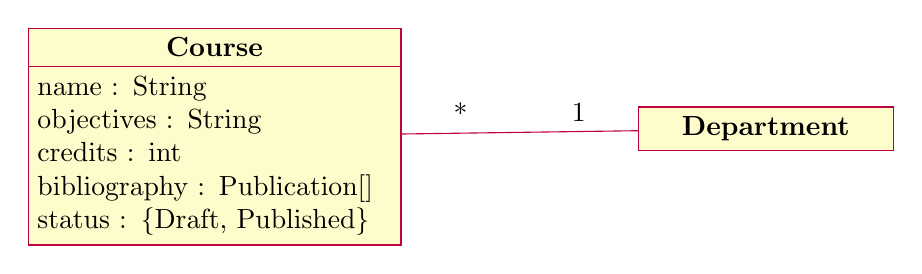
\begin{tikzpicture}

\begin{class}[text width=4.5cm]{Course}{0.5,0}
\attribute{name : String}
\attribute{objectives : String}
\attribute{credits : int}
\attribute{bibliography : Publication[]}
\attribute{status : \{Draft, Published\}}
\end{class}

\begin{class}[text width=3cm]{Department}{7.5,-1}
\end{class}

\association{Department}{}{1}{Course}{}{*}

\end{tikzpicture}

\caption{Domain Model with state representation} 
\label{fig:courseDomainState}

\end{figure}

All the approaches presented above are deemed unacceptable, since they
require explicit intervention by the programmer. 

This section should present only general difficulties, each individual
sub-section of (3)

\subsection{Applications of LLTs}

Long-Lived Transactions are useful in many contexts, 

\subsubsection{Database Management Systems}

*Explain how long-lived transactions are typically implemented in DBMS's*

\subsubsection{Workflow Systems}

Workflow Managements Systems have seen many developments over the last
years.

Workflow systems 

*Explain common use cases of LLT's on Workflow systems, and why are
they so important*


\section{Related Work}

In this section I describe the various topics in which an attempt to
solve the problem of Long Lived Transactions has been made, namely
Database Management Systems, Workflow Systems and Object Oriented
Transactional Systems.

Also, due to its relevance regarding the
solution described in section 4, I briefly present Software
Transactional Memories, and how they cope with short lived transactions.

\subsection{Database world}

*Mention classic books*

*Mention Martin Fowler's patterns \cite{fowler2003patterns}*

*Relaxation of transactional properties*

*Several Papers: \cite{hagmann1991implementing} \cite{garcia1987sagas}
\cite{salem1989altruistic}

*Talk about isolation levels*

*Mention that the best implementations of LLT's at the database level
provide only Serializability at best*

\subsection{Workflow Management Systems}

*Sagas* \cite{garcia1987sagas}

\cite{798492}

*Compensations*

*Exception Handling systems*

*Explain why those solutions are not good, since they *may* break ACI
of the ACID model*

\subsection{Object-Relational Mappings}

*Talk about how ORM's handle transactions, i.e. Hibernate*

\subsection{Object-Oriented}

*Talk about ORM's in Object Oriented systems, such as Hibernate*

*Talk about the Fenix Framework, how it implements a Persistent STM,
mention that the Framework brings Strict Serializability to a
'transparent' programming model* \cite{fernandes2011strict} 
\cite{guerraoui2008correctness} \cite{cachopo2006versioned}

*Talk about how this project aims at extending the FF model to support LLT's*

\subsection{STM's}
\label{sec:stm}


\section{Solution Architecture}

In this section I will describe the architecture of my proposed
solution, as well as a small introduction to the Fénix Framework
\cite{fernandes2011strict}, in which it will be implemented.

\subsection{Fenix Framework}

STMs, PSTMs, DML

\ref{sec:stm}

Describe that the solution will be build on top of the Fenix Framework
core, plus JVSTM, making it agnostic to the specific persistence
backend in use. 

\subsection{Transactional Contexts}

The basic building block 

\subsection{Programming Model}

\lstset{language=Java,frame=single,caption={Sample
  implementation of a method that runs inside a Long Lived
  Transaction}}
\begin{lstlisting}

public CourseCreation(Department department) {
  this.setDepartment(department);
  this.setNewCourse(new Course());
  department.addCourse(this.getNewCourse());
}

@Step
public void createNewCourse(String courseName) {
  this.getNewCourse().setName(courseName);
}

@Step(last = true)
public void setBibliography(Publication[] bibliography) {
  this.getNewCourse().setBibliography(bibliography);
}
\end{lstlisting}

\section{Evaluation}

The final evaluation of this project will be measured in terms of:
- Programmer effort needed to use LLT's
- Performance, throughput, Commit/Abort ratios, interleaving LLTs with
'regular' transactions

\section{Conclusion}

\bibliography{thesis.bib}
\bibliographystyle{plain}
\end{document}
